\section{Multimedia data}


\subsection{The shift to wards multimedia data}

\begin{frame}{An old problem\ldots}
  \begin{itemize}
  \item Quantiative content analysis can be applied not only to text, but also to visuals \parencite[e.g.,][]{Bock2011}
  \item Not often done: labor intensive, (easy) data availability, \ldots
  \item Yet, more and more important in online settings \parencite[e.g.,][]{Araujo2020b}
  \end{itemize}
\end{frame}


\question{Maybe computational methods can help?}

\begin{frame}{Yes, they can! }
  A recent turn towards automated content analysis of visual content -- incluing a whole special issue on ``images as data'' in CCR \parencite{Casas2022}:
 
  \begin{enumerate}
  \item Images become more important (e.g., Instagram)
  \item More images available to social scientists (not only social media, but also repositories, archives, \ldots)
  \item New computational methods available
  \end{enumerate}
\end{frame}



\begin{frame}{Yet, not as mainstream as compuational textual methods}
``Moreover, [\ldots] there are
starting costs to learning [\ldots]  computer vision
methods, given that the jargon is often very computer-science and machine-
learning specific, and state-of-the-art libraries and packages are available
mostly in Python while social scientists are often more used to working
in the R programming language. Thus
the special issue aims to lower
start-up costs for scholars interested in using images-as-data methods in
their research.''
\parencite[p.~3]{Casas2022}
\end{frame}

\begin{frame}[standout]
And yet, as we'll see, it's not that big a leap from what we already know!
\end{frame}


\begin{frame}{Some examples}
  \begin{block}{\cite{Chen2022}}
    \textbf{Can we detect conspiracy videos?}

    It seems we can, based (also) on visual features like contrast and brightness.

    Techniques: Manual feature extraction + classical ML
  \end{block}
\end{frame}


\begin{frame}{Some examples}
  \begin{block}{\cite{Jurgens2022}}
    \textbf{How are age and gender represented on German TV?}

    There seems to be discrimination against women and elderly

    Techniques: Deep learning using pre-trained models
  \end{block}
\end{frame}



\begin{frame}{Some examples}
  \begin{block}{\cite{Joo2022}}
    \textbf{How do politcians represent themselves visually in the media?}

    It seems there are party and gender differences
    
    Techniques: Commercial API
  \end{block}
\end{frame}


\begin{frame}[standout]
  Let's have a look at the table of contents of the special issue:
  \url{https://computationalcommunication.org/ccr/issue/view/8}
\end{frame}

\begin{frame}{Latest trends}
  \begin{itemize}
  \item moving images
  \item combining text and visuals
  \item really hot: Transformers\footnote{Think: a more fancy thing than embeddings that also takes into account that the same word can have a different meaning in different contexts} that model them simultaneously (!!!): ``we present data2vec, a framework that uses the same learning method for either speech, NLP or computer vision. The core idea is to predict latent representations of the full input data'' \parencite{Baevski2022}
  \end{itemize}

\end{frame}



\question{But how do we do all of this? (not data2vec, that's for another time\ldots)}


\subsection{Representing multimedia data}

\begin{frame}{Two types of pictures}
  \begin{block}{Pixel graphics (also called bitmap or raster graphic)}
    \begin{itemize}
    \item a matrix of pixels ($\approx$ square dots) of a color
    \item therefore, loosing quality when scaling (especially  up)
    \item photos, screenshots, \ldots
    \item jpg, png, tiff, \ldots
    \end{itemize}
  \end{block}
\end{frame}

\begin{frame}{Two types of pictures}
  \begin{block}{Vector graphics}
    \begin{itemize}
    \item geometric shapes
    \item therefore, fully scalable
    \item drawings, plots, \ldots
    \item svg, eps, \ldots
    \end{itemize}
  \end{block}
  \pause

  \textbf{We can easily convert vector graphics to pixel graphics -- the other way around only approximately (or not at all)}
\end{frame}


\question{Not focus of today, but important: How would you store graphs for a report you want to publish?}



\begin{frame}{Our focus today}
  \begin{itemize}
  \item We focus on pixel graphics
  \item Note that moving images are just a series of pixel graphics! (traditional movies: 24 per second)
  \item Hence, the techniques discussed today can be applied to (stills from) films as well
  \end{itemize}
\end{frame}


\question{If pixel graphics are just a series of colored points, do we need something like the vectorizer we needed to transform words to numbers?}


\begin{frame}{Representing pixel graphics}
  \begin{block}{Grayscale images}
    \begin{itemize}
    \item If the picture is $200\times 300$ pixel, we have a two-dimensional matrix with $200\times 300 = 60,000$ pixels
    \item With a color depth of 1 byte = 8 bit = $2^8=256$, each of these pixels is an integer between 0 and 255
    \item \textbf{Two dimensions instead of one (for text)} -- but we can \emph{flatten} the matrix to a one-dimensional vector (``vectorize'' it, if you want\ldots) (in this case, of length 60,000)
    \end{itemize}
  \end{block}
\end{frame}


\begin{frame}{Representing pixel graphics}
  \begin{block}{Color images (RGB)}
    \begin{itemize}
    \item Per pixel, we now have three color values (Red, Green, Blue) instead of one (Gray)
    \item Hence, our matrix becomes three-dimensional: $200\times 300\times 3 = 180,000$ integers between 0 and 255
    \end{itemize}
  \end{block}
\end{frame}
  

\begin{frame}{What can we do with images in Python?}
  \begin{itemize}
  \item PIL (Pillow), the Python Image Library, provides many typical image operations (reading, displaying, cropping, color transformations)
  \item That's cool for batch processing (a for-loop and you can resize thousands of images\ldots)
  \item But more imporantly: \textbf{It's just a vector/matrix of integers, so we can do machine learning just like we did before!}
  \end{itemize}
\end{frame}

  

\subsection{Classic SML}

\begin{frame}{First approach}
  \begin{itemize}
  \item If each picture is just a vector of integers, scikit-learn works \emph{exactly the same} as for survey data (Chapter 8) or text (Chapter 11).
  \item Typical example: recognizing hand-written characters with a Random Forest (Example 14.10) or a Support Vector Machine\footnote{\url{https://scikit-learn.org/stable/auto\_examples/classification/plot\_digits\_classification.html}}
  \end{itemize}
\end{frame}


\begin{frame}[fragile]{This is impressive!}
\begin{lstlistingoutputtiny}
Classification report for classifier SVC(gamma=0.001):
              precision    recall  f1-score   support

           0       1.00      0.99      0.99        88
           1       0.99      0.97      0.98        91
           2       0.99      0.99      0.99        86
           3       0.98      0.87      0.92        91
           4       0.99      0.96      0.97        92
           5       0.95      0.97      0.96        91
           6       0.99      0.99      0.99        91
           7       0.96      0.99      0.97        89
           8       0.94      1.00      0.97        88
           9       0.93      0.98      0.95        92

    accuracy                           0.97       899
   macro avg       0.97      0.97      0.97       899
weighted avg       0.97      0.97      0.97       899
\end{lstlistingoutputtiny}
\tiny{\url{https://scikit-learn.org/stable/auto\_examples/classification/plot\_digits\_classification.html}}

\end{frame}


\question{Can you explain why this works?}


\begin{frame}{The intuition behind it}
  If the images are cropped and resized equally (!)\ldots

  \vspace{1cm}
  
  \ldots then the pixels in the center should be white for a 0 but dark for a 8.
\end{frame}


\question{Can you name tasks for which you think this would \emph{not} work?}




\subsection{Deep Learning}

\question{Do you remember what the reason for using deep learning in text classification was?}

\begin{frame}{Say we want to recognize whether an image is a cat or a dog\ldots}
  \begin{itemize}
  \item Can we really say that the color of a pixel maps directly to the ``catness'' or ``dogness'' of the picture?
  \item Or should it not rather be about their fur, the shape of the ears, \ldots
  \item But it seems impossible to engineer these features by hand :-(
  \end{itemize}

  \pause

  Let's use a deep neural network to learn them!
\end{frame}



\question{Are you really seriously interested in classifying dogs and cats? There are many tutorials, e.g. here: \tiny{\url{https://machinelearningmastery.com/how-to-develop-a-convolutional-neural-network-to-classify-photos-of-dogs-and-cats/}}}

\begin{frame}{How do we do this?}
  \begin{itemize}
  \item For deep learning, we use \texttt{keras} instead of \texttt{scikit-learn}
  \item You need to specify the \emph{architecture} of the network
  \item The process is resource-intensive
  \end{itemize}
\end{frame}


\begin{frame}{Different architectures}
  There are many\ldots, but particularly interesting for us:
  \begin{enumerate}
  \item The multilayer perceptron (MLP): A fully-connected feedforward neural network (see Fig.~\ref{fig:MLP1})
  \item The Convolutional Neural Network (CNN): Layers are not fully connected -- think: regularized versions of MLP
  \end{enumerate}



\end{frame}


\begin{frame}[plain]
\begin{figure}
  \centering
 \begin{neuralnetwork}[height=6]
        \newcommand{\x}[2]{$x_####2$}
        \newcommand{\y}[2]{$\hat{y}_####2$}
        \newcommand{\hfirst}[2]{\small $h^{(1)}_####2$}
        \newcommand{\hsecond}[2]{\small $h^{(2)}_####2$}
        \inputlayer[count=5, bias=true, title=Input\\layer, text=\x]
        \hiddenlayer[count=4, bias=true, title=Hidden\\layer 1, text=\hfirst] \linklayers
        \hiddenlayer[count=4, bias=true, title=Hidden\\layer 2, text=\hsecond] \linklayers
        \hiddenlayer[count=4, bias=true, title=Hidden\\layer 3, text=\hsecond] \linklayers
        \outputlayer[count=1, title=Output\\layer, text=\y] \linklayers
\end{neuralnetwork}
\footnotesize{\caption{Architecture of a multilayer perceptron for binary predictions. The activation function of the output layer is the (logistic) sigmoid function; the other activation functions can be anything (e.g., ReLu) \label{fig:MLP1}}}
\end{figure}
\end{frame}



\begin{frame}[plain]
\begin{figure}
  \centering
 \begin{neuralnetwork}[height=6]
        \newcommand{\x}[2]{$x_####2$}
        \newcommand{\y}[2]{$\hat{y}_####2$}
        \newcommand{\hfirst}[2]{\small $h^{(1)}_####2$}
        \newcommand{\hsecond}[2]{\small $h^{(2)}_####2$}
        \inputlayer[count=5, bias=true, title=Input\\layer, text=\x]
        \hiddenlayer[count=4, bias=true, title=Hidden\\layer 1, text=\hfirst] \linklayers
        \hiddenlayer[count=4, bias=true, title=Hidden\\layer 2, text=\hsecond] \linklayers
        \hiddenlayer[count=4, bias=true, title=Hidden\\layer 3, text=\hsecond] \linklayers
        \outputlayer[count=3, title=Output\\layer, text=\y] \linklayers
\end{neuralnetwork}
\footnotesize{
 \caption{Architecture of a multilayer perceptron for multiclass predictions. The activation function of the output layer is the softmax function (like logistic, but probabilities add up to one); the other activation functions can be anything (e.g., ReLu) \label{fig:MLP2}}}
\end{figure}
\end{frame}


\begin{frame}{Convolutional Neural Networks}
  \begin{itemize}[<+->]
  \item You start with a convolution layer
  \item A convolution is a mathematical operation on two functions\footnote{cross-correlation with one of the functions mirrored around the y-axis}
  \item Think of it as a filter (say, sized $5\times 5$ pixels) that slides over the image
  \item The result goes through a pooling layer that aggregates the outcome (e.g., using the max)
  \item Optionally: More convolution and pooling layers
  \item Finally, one or more fully-connected layers
  \end{itemize}
\end{frame}



\begin{frame}[plain]
\begin{figure}
  \centering
  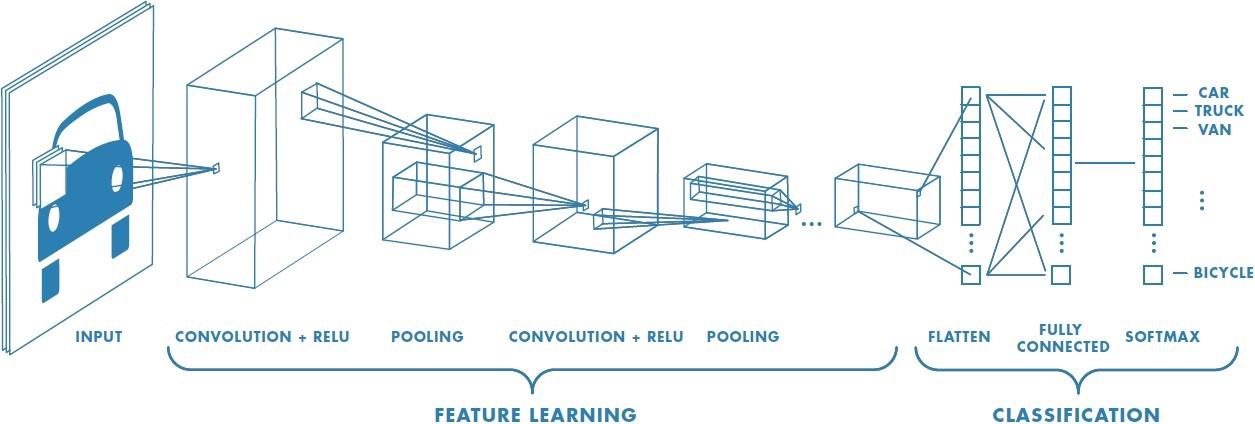
\includegraphics[width=\columnwidth,height=\paperheight,keepaspectratio]{cnn1.jpg}
  \footnotesize{
 \caption{Architecture of a convolutional neural network. Source: \url{https://towardsdatascience.com/a-comprehensive-guide-to-convolutional-neural-networks-the-eli5-way-3bd2b1164a53} \label{fig:CNN1}}}
\end{figure}
\end{frame}


\begin{frame}[plain]
\begin{figure}
  \centering
  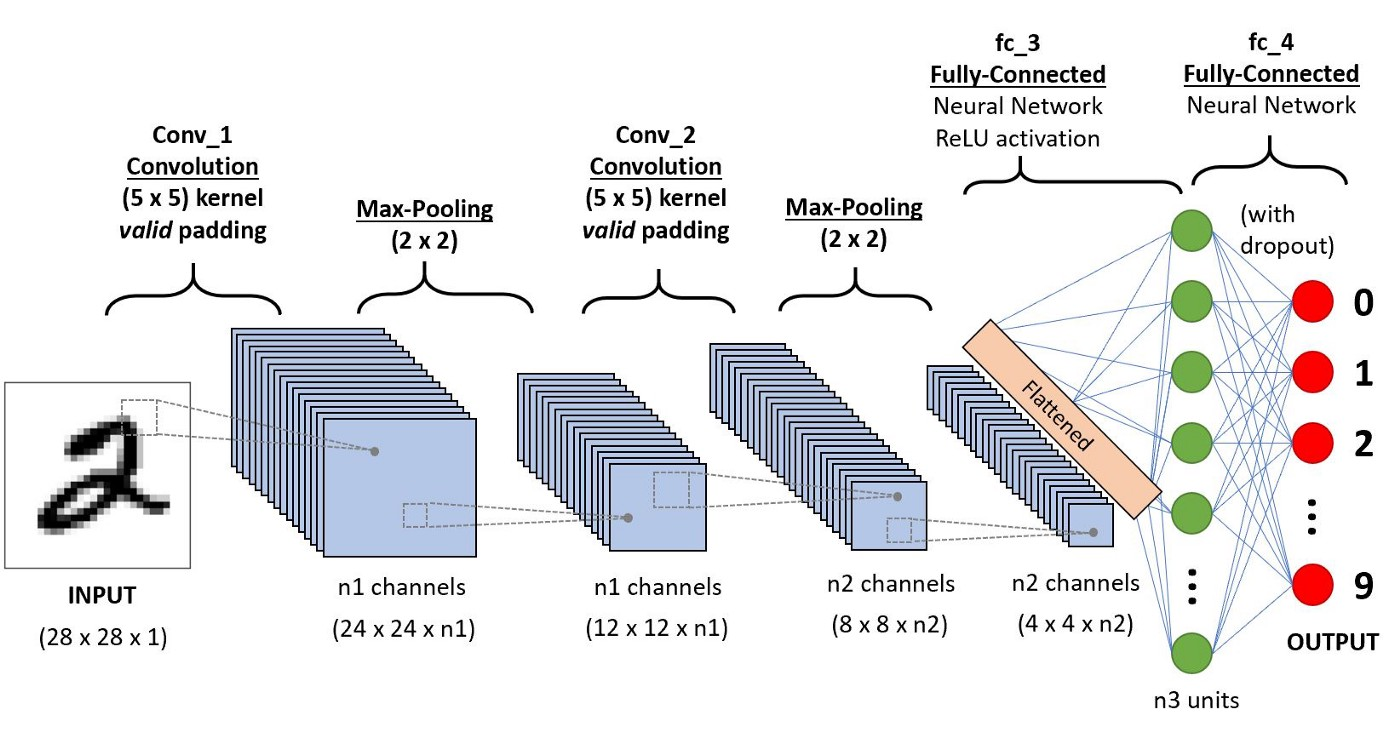
\includegraphics[width=\columnwidth,height=\paperheight,keepaspectratio]{cnn2.jpg}
  \footnotesize{
 \caption{Architecture of a convolutional neural network. Source: \url{https://towardsdatascience.com/a-comprehensive-guide-to-convolutional-neural-networks-the-eli5-way-3bd2b1164a53} \label{fig:CNN2}}}
\end{figure}
\end{frame}

  


\begin{frame}{Convolutional Neural Networks}
  \begin{itemize}[<+->]
  \item CNNs are more modern than MLPs and
  \item Because they integrate a \emph{feature learning} step before the \emph{classification} step, they need less preprocessing (Fig.~\ref{fig:CNN1}
  \item CNNs are more resource-intensive to train
  \end{itemize}
\end{frame}




\begin{frame}{Training your own neural network?}
  If you have a very specific task and an annotated dataset -- sure!

  But:
  \begin{itemize}
  \item Can be \emph{very} resource-intensive
  \item Often, very large amounts of training data needed
  \item There are so many architectures, and you can't possibly know the best ones without being an expert
  \end{itemize}
\end{frame}


\begin{frame}{Training your own neural network?}
  \begin{block}{Solution 0: Just do it ;-)}
Training a MLP if not that difficult (Examples 14.11--14.14)
  \end{block}
\end{frame}



\begin{frame}{Training your own neural network?}
  \begin{block}{Solution 1: Using a pre-trained model}
Just use a CNN that already is trained (Examples 14.14--14.17). Make sure to read up on the specific model you are using.
  \end{block}
\end{frame}

\begin{frame}{Training your own neural network?}
  \begin{block}{Solution 2: Fine-tuning a pre-trained model}
If you have a labeled dataset, you can start with an existing pre-trained model and then fine-tune it with your data (many tutorials online)
  \end{block}
\end{frame}


\begin{frame}{Training your own neural network?}
  \begin{block}{Solution 3: A (commercial) API}
    (next section)
  \end{block}
\end{frame}


  



\subsection{(Commercial) APIs}

\begin{frame}{What is it?}
  \begin{itemize}
  \item You send an image to the API and get a set of labels back
  \item Under the hood: pre-trained neural networks
  \item Very much black box: you have no idea where the labels come from
  \item Prominent players: Clarifai, Google Cloud Vision, Microsoft
  \item Usually paid but often free for small projects and/or academic use
  \end{itemize}

\end{frame}


\begin{frame}{Automated Visual Content Analysis  \parencite{Araujo2020b}}
  \begin{alertblock}{Problem}
The labels do not correspond what one may be theoretically interested in.
  \end{alertblock}

  \pause
  
\begin{block}{Solution}
  \begin{itemize}
  \item Annotate a set of images manually using a codebook
  \item Use the labels provided by the API as features to train a classifier to predict the annotations
  \item Thus, we essentially have transformed the image prediction task to a textual prediction task
  \end{itemize}
\end{block}
\end{frame}



\begin{frame}{Is it difficult to use a computer vision API?}
  \textbf{No.}

All providers provide Python code examples, e.g. \url{https://cloud.google.com/vision/docs/detect-labels-image-client-libraries}
  
\end{frame}



\begin{frame}{Further reading}
  \begin{itemize}
  \item all the articles in the special issue edited by \cite{Casas2022}
  \item a short book by \cite{Webbwilliams2020}
  \item the study by \cite{Araujo2020b}
  \end{itemize}
\end{frame}



\begin{frame}{Final remark}
  The black box nature of (most of) these techniques \emph{is} a big problem from a social-science and epistemological point of view: in particular, known and un-known biases!

As always, but maybe especially here: Never take the outcome as a given -- it needs interpretation and critical reflection!

\end{frame}
